\chapter{Zašto naučnici i dalje nisu razvili vakcinu za HIV}
\section{Uvod}
\subsection{Klasifikacija HIV fenotipa}

1984. godine, američka ministarka zdravlja Margaret Hekler je objavila da će vakcina za HIV biti dostupna u narednih 2 godine. 1997. godine, Bil Klinton je otvorio novi centar za istraživanje na Nacionalnom institutu zdravlja, sa ciljem da se razvije vakcina za HIV. Kompanija Merck je 2005. počela kliničko ispitivanje vakcine za HIV, ali je odustala  posle 2 godine, jer su rezultati pokazali da je vakcina zapravo povećala rizik od dobijanja HIV-a kod nekih primalaca vakcine.

Danas, uprkos ogromnim investicijama i istraživanjima, daleko smo od razvijanja vakcine za HIV, a 35 miliona ljudi žive s tom bolešću. Naučnici su napravili ogroman napredak u razvoju antiretroviralne terapije, koja predstavlja mešavinu lekova koji stabilizuju simptome zaraženog pacijenta. Međutim, ova terapija ne leči sidu i ne može da zaustavi širenje HIV-a tako da ne predstavlja pravu vakcinu za sidu. 

Klasične vakcine protiv virusa su često napravljene od proteina virusa. Ove vakcine stimulišu čovekov imuni sistem da prepozna virusne omotače proteina kao strane, da ih uništi i da sačuva podatke o njima, da bi imuni sistem mogao kasnije da ih identifikuje i iskoreni.

Međutim, virusni omotači proteina HIV virusa mogu biti ekstremno promenljivi, zato što virus mora da mutira brzo da bi preživeo. Virus HIV-a kod neke osobe evoluira vrlo brzo da bi izbegao imuni sistem čoveka. Takođe, uzorci HIV-a uzeti od različitih pacijenata su pokazali da oni imaju podtipove koji se veoma razlikuju. Dakle, uspešna vakcina za HIV mora biti dovoljno širokog spektra da pokrije sve ove različitosti. 

HIV ima samo devet gena i u ovom poglavlju se fokusiramo na \textit{env} gen koji brzo mutira. Protein koji kodira \textit{env} gen ulazi u \textbf{glycoprotein gp120} i \textbf{glycoprotein gp41}.

S obzirom da HIV mutira tako brzo, različiti izolati HIV-a mogu imati različite fenotipe, koji onda zahtevaju različite mešavine lekova. HIV virusi se mogu podeliti na brzo replicirajuće (SI) izolate i sporo replicirajuće NSI izolate. Tokom infekcije, proteini virusa kao što je gp120 koje HIV koristi da uđe u ćelije se prenose do površine ćelije, gde mogu da prouzrokuju da se ta ćelija spoji sa susednom ćelijom. To uzrokuje da desetine ljudskih ćelije spoje svoje ćelijske membrane u jedan veliki, nefunkcionalni syncytium ili u abnormalnu multinukleaturnu ćeliju. Na ovaj način, inficirajući samo jednu ćeliju, biće ubijene mnoge ljudske ćelije.

\subsubsection{Ograničenja u poravnanju sekvenci}

Pre nego što biologičari uopšte mogu da počnu da proučavaju pitanje predviđanja HIV fenotipa koristeći gp120 sekvence, oni se suočavaju sa problemom konstrukcije preciznog poravnanja ovih sekvenci. Čak i jedna pogrešno poravnanje, koje postavlja amino kiselinu na poziciju utičući na SI/NSI fenotip, može prouzrokovati pogrešnu klasifikaciju HIV fenotipa. Iz poglavlja 5, već znamo da je konstrukcija višestrukog poravnanja sekvenci koje divergiraju težak algoritamski problem. 

Problem formulacije višestrukog poravnanja uveden u poglavlju 5 ne pruža adekvatnu translaciju biološkog problema PHV klasifikacije u algoritamski problem. Zbog toga moramo smisliti novu formulaciju problema poravnanja sekvenci koja će dovesti statistički solidne analize gp120 proteina.

\section{Pronalaženje CG ostrva}

Početkom dvadesetog veka, Phoebus Levene je otkrio četiri nukleotida od kojih se sastoji DNK. U to vreme, vrlo malo se znalo o DNK. Zbog toga, Levene je sumnjao da DNK može da čuva genetstke informacije koristeći samo četiri slova i postavio je hipotezu da se u DNK nalazi gotovo jednak broj adenina, citozina, guanina i timina. Jedan vek kasnije, znamo da komplementarni nukleotidi na suprotnim obalama DNK imaju jednaku frekvenciju osnovnog uparivanja, ignorišući ekstremno retke greške osnovnog uparivanja. Međutim, nije tačno da su frekvencije nukleotida približno iste na jednoj obali DNK. Različite vrste imaju različite \textbf{CG-sadržaje}, ili procenat citozina i guanina u genomu.

Mogli bismo očekivati da se svaki od dinukleotida CC, CG, GC, GG u ljudskom genomu javlja sa frekvencijom od 0.21 * 0.21 + 4.41\%. Međutim, frekvencija CG u ljudskom genomu je samo 1\%. Ovaj dinukleotid je toliko redak zbog \textbf{metilacije}.

\begin{definicija}
Metilacija je dodavanje metil (CH3) grupe na citozin (često u okviru CG dinukleotida).
\end{definicija}


Rezultujući metilovani citozin ima tendenciju da deaminuje u timin. Kao rezultat metilacije, CG je najređi dinukleotid u mnogim genomima. Metilacija je često izostavljena u genima u regionima pod nazivom \textbf{CG-ostrva} (CG se često pojavljuje). 

U prvom pokušaju za nalaženje ovakvih gena, kako bismo tražili CG-ostrva? Naivan pristup traženju CG-ostrva bi bio da se pomera prozor kroz genom, proglašavajući prozore sa većom frekvencijom CG, potencijalnim CG-ostrvima. Mane ovog pristupa bi bile iste kao i pri pomeranju prozora da bi se odredio koji novčić je krupije koristio u kom trenutku. Ne znamo koliki će prozor biti i zato nije jasno kako odabrati veličinu prozora za detekciju CG-ostrva. Takođe, različiti prozori mogu klasifikovati iste pozicije u genomu različito.

\section{Nepoštena kockarnica}
\subsection{Kockanje sa Jakuzama}
Japanska kriminalna organizacija pod nazivom jakuza potiče iz od grupe putujućih kockara iz 18. veka koji su se nazivali bakut ("jakuza" je naziv za gubitničku ruku u Japanskoj kartaškoj igri). Jedna od najpopularnijih igara koju su bakuto organizovali u svojim kazinoima se zvala Čo-Han. U ovoj igri, koja se bukvalno prevodi kao "jednake šanse", krupije baca dve kockice, a igrač se kladi na to dali će suma kockica biti paran ili neparan broj.

Iako je igranje Čo-Han igre u jakuzinim kockarnicama veoma zanimljivo, možemo takođe igrati i igru koja se zove "glava ili pismo", tako što se baca novčić u vazduh i pogađa se ishod. Pretpostavimo da se iz nekog razloga više ljudi kladi na pismo nego na glavu u ovoj igri. U tom slučaju bi nepošten krupije mogao da iskoristi otežani novčić koji ima veću verovatnoću da padne na glavu nego na pismo. Mi ćemo pretpostaviti da otežani novčić ima verovatnoću da padne na glavu 3/4.

\textbf{Pitanje:} Recimo da igramo igru pismo ili glava 100 puta, i novčić padne na glavu 63 puta. Da li možemo da kažemo da krupije vara? Da li je korišćen fer ili otežan novčić?
\textbf{Nagoveštaj}: 63 je bliže 75
nego 50!

Pitanje nije dobro formulisano, jer bilo koji novčić može da proizvede bilo koji niz bacanja. Da li možemo da utvrdimo koji novčić
je verovatnije korišćen? Zapišimo verovatnoću padanja pisma ("T") i glave ("H") za fer novčić (F) kao: 
\begin{equation}
Pr_F("H") = 1/2     Pr_F("T") = 1/2
\end{equation}
i verovatnoća otežanog novčića (B):
\begin{equation}
Pr_B("H") = 3/4     Pr_B("T") = 1/4
\end{equation}
Kako su bacanja novčića nezavisni događaji, verovatnoća da će $ n $ bacanja fer novčića proizvesti dati niz $ x= x_1x_2...x_n $ sa $ k $ pojavljivanja glave je:
\begin{equation}
Pr(x|F) = {\displaystyle \prod_{i=1}^n Pr_F(x_i)} = (1/2)^n.
\end{equation}
Verovatnoća da će otežani novčić da proizvede isti niz je:
\begin{equation}
Pr(x|B) = {\displaystyle \prod_{i=1}^n Pr_B(x_i)} = (1/4)^{(n-k)} \cdot (3/4)^k = 3^k/4^n.
\end{equation}
Ako je Pr(x$|$F) $>$ Pr(x$|$B), onda je veća verovatnoća da je krupije koristio fer novčić, a ako je Pr(x|F) $<$ Pr(x|B), onda je obrnuto.
Kada su jednaki Pr(x$|$F) = Pr(x$|$B) tada je:
\begin{equation}
(1/2)^n = (1/4)^{(n-k)} \cdot (3/4)^k \rightarrow 2^n = 3^k \rightarrow k = {\log_2 3} \cdot n \rightarrow k \approx 0.632 \cdot n
\end{equation}
Dakle ukoliko je mera odnosa $ k/n < 1/{\log_2 3}$, tada je i Pr(x$|$F) $>$ Pr(x|B).
Iako je 63 bliže 75 nego 50, fer novčić će sa većom verovatnoćom dati 63 glave u 100 bacanja.

\subsection{Dva novčića u krupijeovom rukavu}
U bakuto kockarnicama, Čo-Han krupije bi skinuo svoju majicu u toku igre, kako bi skinuo sa sebe sumnju da mulja sa kockicama. Mi ćemo ipak pretpostaviti da u igri glava ili pismo, nepošteni krupije nosi majicu i drži oba novčića u svom rukavu i može da ih neprimetno menja u bilo kom trenutku. Pošto ne želi da bude uhvaćen kako zamenjuje novčiće, on ih menja samo povremeno, pretpostavimo sa verovatnoćom 0.1 nakon svakog bacanja. 

\textbf{Pitanje:} Nakon niza bacanja novčića, možemo
li reći kada je krupije koristio fer coin a
kada otežani novčić?

\begin{problem}[Kazino problem.]
Za dati niz bacanja novčića,
odrediti kada je krupije koristio fer a kada
otežani novčić.
\begin{itemize}
\item Ulaz: Niz $ x = x_1 x_2 \ldots x_n $ bacanja dobijenih
od novčića F (fer) i B (otežani).
\item Izlaz: Niz $ \pi = \pi_1 \pi_2 \ldots \pi_n $, gde je svako $ \pi_i $
jednako ili F ili B što znači da je $ x_i $
dobijeno bacanjem fer ili otežanog novčića,
redom.
\end{itemize}
\end{problem}

Nažalost, ni ovo nije dobro definisan problem. Svaki ishod bacanja novčića može biti dobijen bilo kojom permutacijom fer i
otežanog novčića! HHHHH je moglo biti dobijeno od BBBBB,
FFFFF, FBFBF, itd.

Neophodan je način za ocenjivanje različitih scenarija: BBBBB, FFFFF,
FBFBF, itd. zavisno od toga koliko je svaki od njih verovatan.

Kako da ispitamo i ocenimo $ 2^n $ mogućih scenarija? 

Jedan pristup ovom problemu da pogodimo koji novčić je verovatnije krupije koristio u svakom bacanju je da uzmemo "okvir prozora" (dužine $ t < n $) duž niza bacanja $ x = x_1...x_n $ i da izračunamo meru odnosa fer i otežanog novčića (kao u gornjem primeru) u okviru svakog prozora. Ukoliko je mera odnosa u okviru prozora manja od nule, onda je veća verovatnoća da krupije koristi otežani novčić u okviru prozora, inače je obrnuto.

Postoji dva problema sa metodom "okvira prozora". Prvo je da nemamo vidan način da odaberemo dužinu okvira prozora. Drugo, okviri prozora koji se preklapaju mogu klasifikovati isti ishod uzrokovan i otežanim i fer novčićem. Na primer, ako je $x$ = "HHHHHTTHHHTTTTT", onda prozor $x_1...x_{10}$ = "HHHHHTTHHH" ima negativnu meru odnosa, a onda prozor $ x = x_6...x_{15}$ = "TTHHHTTTTT" ima pozitivnu meru odnosa. Koji je novčić krupije koristio na bacanjima $x_6...x_{10}$ ?

\section{Skriveni Markovljevi modeli}
\subsection{Od bacanja novčića do Skrivenog Markovljevog Modela}

Naš cilj je razvijemo koncept koji modeluje nepoštenog krupijea i potragu za CG-ostrvima u genomu. Krupijea možemo posmatrati kao
mašinu koja ima $ k $ skrivenih stanja ($ F $ i $ B $). U svakom koraku, emituje simbol (H ili T) iz jednog od svojih skrivenih stanja. Dok je u određenom stanju, mašina donosi dve odluke:
\begin{itemize}
    \item Koji simbol ću emitovati?
    \item  U koje skriveno stanje ću nakon toga preći?
\end{itemize}

Mašina odgovara na prvo pitanje tako što izabere proizvoljan broj između stanja $ F $ i $ B $, sa verovatnoćom 0.9 da će ostati u trenutnom stanju i verovatnoćom 0.1 da će promeniti stanje. Mašina odgovara na drugo pitanje tako što bira između simbola H i T sa verovatnoćama koje zavise od toga u kom stanju je trenutno. Naš cilj je da zaključimo koja je najverovatnija sekvenca stanja mašine analizirajući sekvence simbola koje emituje.

Na ovaj način smo pretvorili krupijea u apstraktnu mašinu koja se zove \textbf{Skriveni Markovljev Model} (HMM). Razlika između mašine za bacanje novčića i generalnog koncepta HMM-a je što će HMM kasnije imati proizvoljan broj stanja i može da ima proizvoljnu distribuciju verovatnoća, odlučujući u koje stanje da pređe i koje simbole da emituje.  

\subsection{HMM dijagrami}

HMM se definiše kao skup četiri objekta:
\begin{itemize}
    \item azbuka emitovanih simbola $ \Sigma $ (H i T)
    \item skup skrivenih stanja ($ F $ i $ B $)
    \item Matrica verovatnoće prelaska: $ Transition $ = ($ transition_{l,k} $): $ |States| \times |States| $ matrica
    \textbf{verovatnoća prelaska} (iz stanja $ l $ u stanje $ k $)
    \item Matrica emisionih verovatnoća: $ Emision $ = ($ emision_k(b) $): $ |States| \times |\Sigma| $ matrica
    \textbf{emisionih verovatnoća} (emitovanje simbola $ b $ u stanju $ k $)
\end{itemize}

Kao što je prikazano na slici \ref{slika: hmm}, HMM se može prikazati kao HMM dijagram, graf gde je svako stanje predstavljeno jednim punim čvorom. Usmerene pune grane povezuju svaki par čvorova, kao i svaki čvor sa sobom. Svaka takva grana je obeležena verovatnoćom prelaska iz jednog stanja u drugo. HMM dijagram takođe ima i isprekidane čvorove koji predstavljaju simbole azbuke $ \Sigma $ i isprekidanje grane koje povezuju svako stanje sa svojim isprekidanim čvorom. Svaka takva grana je obeležena verovatnoćom da će HMM emitovati taj simbol dok je u tom stanju.

\begin{figure}[H]
\centering
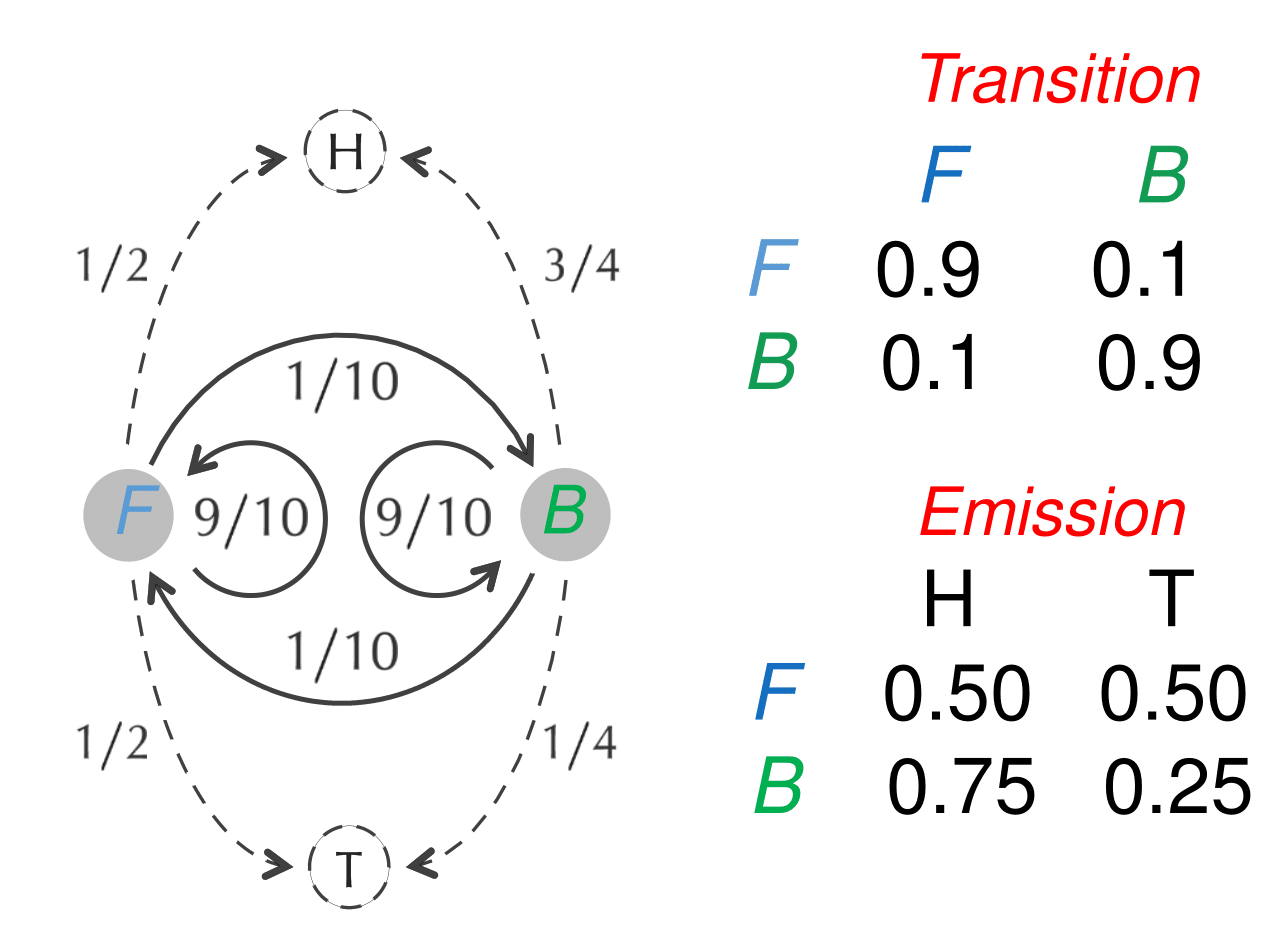
\includegraphics[width=0.5 \textwidth]{poglavlja/10/slike/HMM-dijagram.png}
\caption{HMM dijagram}
\label{slika: hmm}
\end{figure}



\begin{definicija}
    \textbf{Skrivena putanja} je niz $ \pi = \pi_1, ... , \pi_n $ stanja kroz koje HMM prolazi.
\end{definicija}

Slika \ref{slika: hmm} prikazuje primer gde nepošteni krupije HMM proizvodi sekvencu $ x $ = ``THTHHHTHTTH`` sa skrivenom putanjom $ n = FFFBBBBBFFF $. Fer novčić je korišćen za prva tri bacanja i za poslednja tri bacanja, a otežani novčić se koristi za pet bacanja između.

Uvedimo sledeće jednakosti:

\begin{itemize}
    \item $ Pr(x, \pi) $: zajednička verovatnoća da dati HMM
    polazi kroz stanja $ \pi $ i emituje nisku $ x = x_1 x_2
    . . . x_n $.
    \item $ Pr(x|\pi) $: uslovna verovatnoća da HMM
    emituje nisku $ x $ nakon prolaska kroz skrivenu putanju $ \pi $.
    \item $ Pr(x, \pi) = Pr(x|\pi) * Pr(\pi) $
\end{itemize}

Da bi se izračunalo $ Pr(x, \pi) $, prvo moramo da izračunamo $ PR(\pi) $. Neka $ Pr(\pi_i \rightarrow \pi_{i+1}) $ označava verovatnoću prelaska HMM-a iz stanja $ \pi_i $ u stanje $ \pi_{i+1} $. Verovatnoća za $ \pi $ je jednaka proizvodu verovatnoća prelaska 

\begin{equation}
    Pr(\pi) = {\displaystyle \prod_{i=1}^n Pr(\pi_{i-1} \rightarrow \pi_i)} = {\displaystyle \prod_{i=1}^n transition_{\pi_{i-1}, \pi_i}}
\end{equation}

\begin{problem}[Problem verovatnoće skrivene putanje. ]
	Izračunati verovatnoću skrivene putanje HMM-a.\\
	Ulaz: Skrivena putanja $ \pi $ i model HMM ($ \Sigma $,$ States,Transition,Emission $). \\
	Izlaz: Verovatnoća date putanje, $ Pr(\pi) $.
\end{problem}

Da bismo izračunali $ Pr(x|\pi) $ za neki HMM, označićemo sa $ Pr(x_i|\pi_i) $ verovatnoću emitovanja $ emission_{\pi_i}(x_i) $ da je $ x_i $ emitovan kada je HMM bio u stanju $ \pi_i $. Ko rezultat toga, za neku putanju $ \pi $, HMM emituje string $ x $ sa verovatnoćom jednakom proizvodu verovatnoća emitovanja na toj putanji,

\begin{equation}
    Pr(x, \pi) = {\displaystyle \prod_{i=1}^n Pr(x_i|\pi_i)} = {\displaystyle \prod_{i=1}^n emission_{\pi_i}(x_i)}    
\end{equation}

\begin{problem}[Problem verovatnoće ishoda za datu skrivenu putanju]
	Izračunati verovatnoću da dati HMM emituje datu nisku za datu skrivenu putanju.\\
	Ulaz:  Niska $ x=x_1, ..., x_n $ koju emituje dati HMM($ \Sigma, States, Transition, Emission $) i skrivena putanja $ \pi = \pi_1, ..., \pi_n. $\\
	Izlaz:  Uslovna verovatnoća $ Pr(x|\pi) $ da će dati HMM emitovati nisku $ x $ prateći skrivenu putanju $ \pi $.
\end{problem}

\section{Problem dekodiranja}
\subsection{Viterbi graf}

\begin{problem}[Problem dekodiranja]
    Naći optimalnu skrivenu putanju sa kojom je dati HMM emitovao datu nisku.\\
    Ulaz: Niska $ x = x_1 . . . x_n $ koju emituje HMM($ \Sigma, States, Transition, Emission $).\\ 
    Izlaz: Putanja $ \pi $ koja maksimizuje verovatnoću $ Pr(x,\pi) $ po svim mogućim putanjama $ \pi $ za ovaj HMM.    
\end{problem}

Da bi rešio problem dekodiranja, Andrew Viterbi je koristio Menhetn graf inspirisan HMM-om. Za HMM koji emituje string od $ n $ simbola $ x = x_1...x_n $, čvorovi HMM-ovog Viterbi grafa se dele na |States| vrsta i $ n $ kolona (slika \ref{slika: menhetn}). Dakle, čvor $ (k, i) $ reprezentuje stanje $ k $ i $ i $-ti emitovani simbol. Svaki čvor je povezan sa svim čvorovima iz kolone s njegove desne strane; grana koja povezuje $  (l, i-1) $ sa $ (k, i) $ odgovara prelasku iz stanja $ l $ u stanje $ k $ (sa verovatnoćom $ transition_{l, k}$) i zatim emitovanju simbola $ x $ (sa verovatnoćom $ emission_k(x_i)$).Kao rezultat toga, sve putanje koja povezuje čvor u prvoj koloni Viterbi grafa sa čvorom u poslednjoj koloni, odgovara skrivenoj putanji $ \pi = \pi_1...\pi_n$.

\begin{figure}[H]
\centering
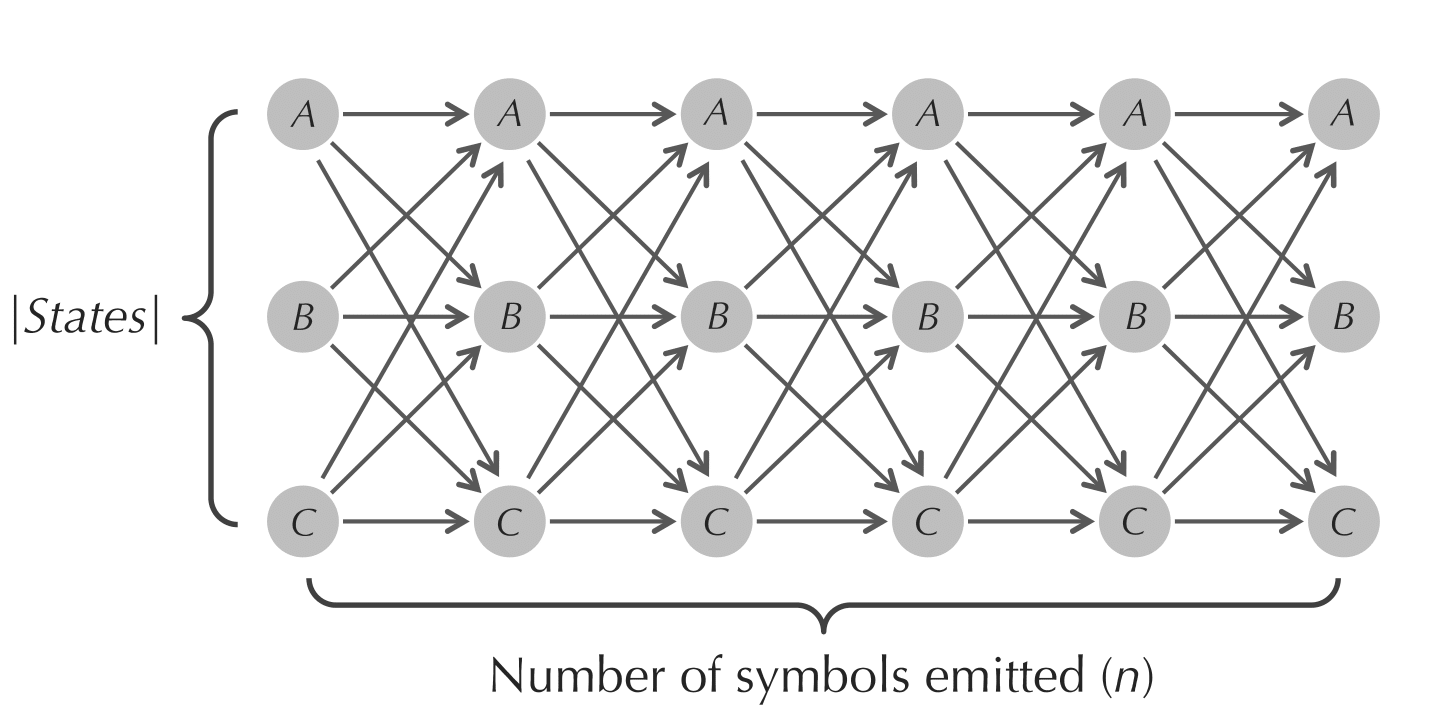
\includegraphics[width=0.8\textwidth]{poglavlja/10/slike/Menhetn_graf.png}
\caption{Menhetn graf za problem dekodiranja}
\label{slika: menhetn}
\end{figure}



Težina grane koja povezuje $ (l, i-1) $ i $ (k, i) $ u Viterbi grafu je jednaka

\begin{equation}
    Weight_i(l, k) = transition_{\pi_i, \pi_{i-1}}*emission_{\pi_i}(x_i)
\end{equation}

Zatim, definišemo \textbf{proizvod težina} putanja u Viterbi grafu, kao proizvod težina njegovih grana. Za putanju od najlevlje kolone do najdesnije(da li se ovo kaže ovako ili sam nepismen?) kolone u Viterbi grafu koja odgovara skrivenoj putanji $ n $, ovaj proizvod je jednak proizvodu $ n-1 $ članova,

\begin{equation}
{\displaystyle \prod_{i=2}^n transition_{\pi_i, \pi_{i-1}}*emission_{\pi_i}(x_i)} = {\displaystyle \prod_{i=1}^{n-1}  Weight_i(l, k)}.
\end{equation}

\subsection{Viterbi algoritam}

Primenićemo algoritam dinamičkog programiranja da bismo rešili problem dekodiranja. Prvo, definišimo $ s_{k, i} $, što predstavlja proizvod težina optimalne putanje (putanje sa najvećom težinom proizvoda) od \textit{izvora} do čvora $ (k, i) $. Viterbi algoritam je zasnovan na činjenici da prvih $ i-1 $ grana optimalne putanje od izvora do $ (k, i) $ moraju formirati optimalnu putanju od izvora do $ (l, i-1) $ za neko (nepoznato) stanje $ l $. Ovo zapažanje proizvodi sledeću jednačinu:

\begin{equation}
\begin{aligned}
    s_{k, i} &= {\displaystyle \max_{all\,states\,l} \{s_{l, i-1} \cdot (weight\,of\,edge\,between\,nodes\,(l, i-1)\,and\,(k, i))\}} \\
    & = \max_{all\,states\,l} \{s_{l, i-1} \cdot Weight_i(l, k)\}\\
    & = \max_{all\,states\,l} \{s_{l, i-1} \cdot transition_{\pi_{i-1},\pi_i} \cdot emission_{\pi_i}(x_i)\}
\end{aligned}
\end{equation}

\subsection{Brzina Viterbi algoritma}

Možemo da posmatramo problem dekodiranja kao još jednu isntancu problema najduže putanje u DAG problemu iz 5. poglavlja, zato što putanja $ \pi $ koja maksimizira proizvod težina $ {\displaystyle \prod_{i=1}^{n}  Weight_i(\pi_{i-1}, \pi_i)} $ takođe maksimizira logaritam ovog proizvoda,  koji je jednak $ {\displaystyle \sum_{i=1}^{n}  log(Weight_i(\pi_{i-1}))} $. Prema tome, možemo da zamenimo težine svih grana u Viterbi grafu njihovim logaritmima. Nalaženje najdužeg puta u rezultujućem grafu će odgovarati putanji maksimalnih težina proizvoda u originalnom Viterbi grafu. Iz ovog razloga, vreme izvršavanja Viterbi algporitma je linearno u odnosu na broj grana u Viterbi grafu. Broj ovih grana je $ |States|^2 \cdot n $ gde je $ n $ broj emitovanih simbola.

U praksi, mnogo HMM-ova ima \textbf{zabranjene prelaze} između nekih stanja. Za takve prelaze, možemo da obrišemo odgovarajuće grane iz HMM dijagrama (slika \ref{slika: viterbi_1}). Ova operacija dovodi do ređeg Viterbi grafa (slika \ref{slika: viterbi_2}), što dovodi do smanjenja vremena izvršavanja Viterbi algoritma, s obzirom da je vreme izvršavanja algoritma za pronalaženje najduže putanje u DAG-u linearno u odnosu na broj grana u tom DAG-u.

\begin{figure}[H]
\centering
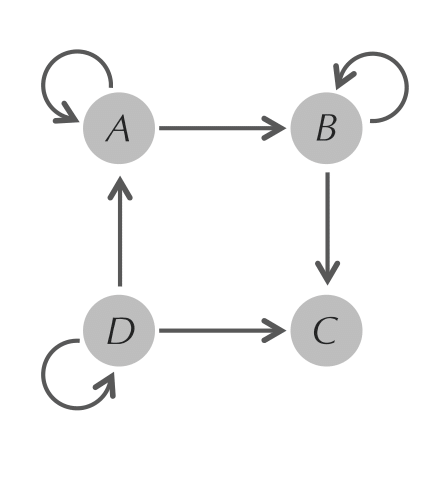
\includegraphics[width=0.3\textwidth]{poglavlja/10/slike/brzina_Viterbi_1.png}
\caption{HMM dijagram sa nekim zabranjenim stanjima kao npr. od A do D ili od C do samog sebe}
\label{slika: viterbi_1}
\end{figure}

\begin{figure}[H]
\centering
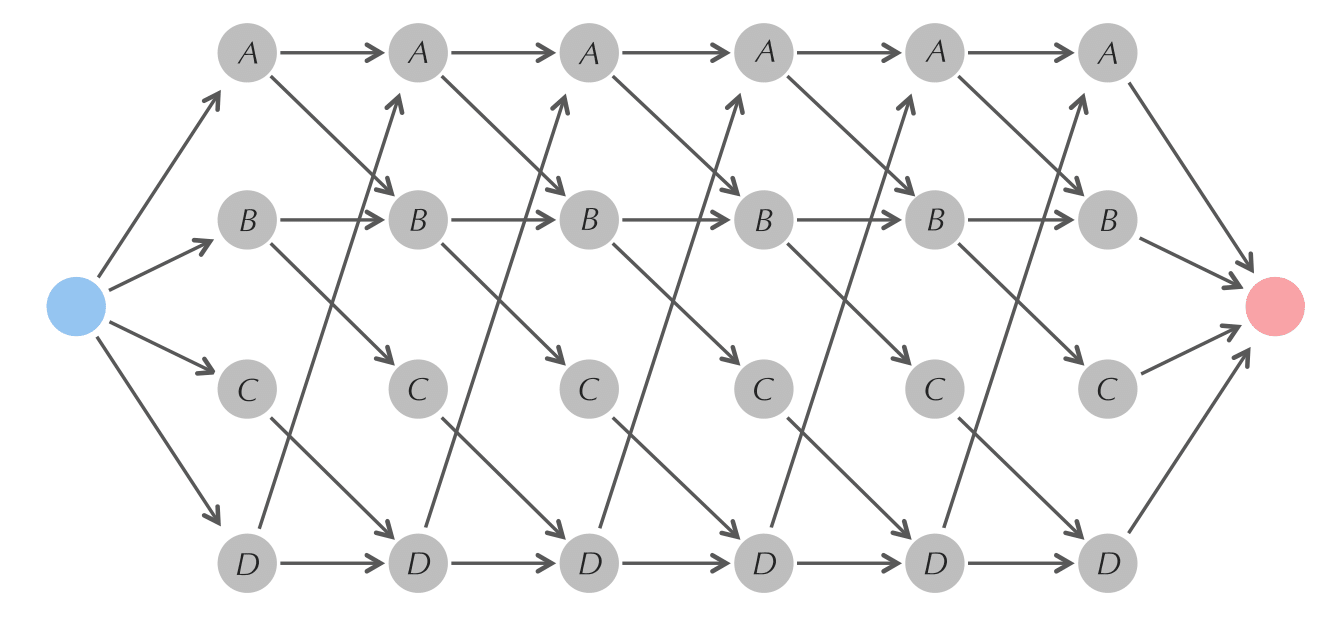
\includegraphics[width=0.8\textwidth]{poglavlja/10/slike/brzina_Viterbi_2.png}
\caption{Viterbi graf za HMM sa prethodne slike koji emituje string dužine 6}
\label{slika: viterbi_2}
\end{figure}

\section{Računanje najverovatnijeg ishoda HMM-a}

Dinamičko programiranje nam pomaže da odgovorimo na pitanje proširivanja HMM-a i preko najverovatnije skrivene putanje. Mi možemo da izračunamo verovatnoću $ Pr(\pi) $ skrivene putanje $ \pi $. Ali šta je sa $ Pr(x) $, koja je verovatnoća da HMM emituje string $ x $?

\begin{problem}[Problem verovatnoće ishoda]
    Izračunati verovatnoću da HMM emituje datu nisku.\\
    Ulaz: Niska $ x = x_1 . . . x_n $ koju emituje HMM($ \Sigma, States, Transition, Emission $).\\ 
    Izlaz: Verovatnoća $ Pr(x) $ da model HMM emituje nisku $ x $.    
\end{problem}

Već smo zaključili da je $ Pr(x) $ jednak sumi $ Pr(x, \pi) $ za sve skrivene putanje $ \pi $. Međutim, broj putanja u Viterbi grafu je eksponencijalan u odnosu na broj emitovanih stringova $ x $, tako da možemo da koristuimo dinamičko programiranje kao brži način da izračunamo $ Pr(x) $.

Neka je $ forward_{k, i} $ proizvod svih putanja od \textit{izvora} do čvora $ (k, i) $ u Viterbi grafu; treba uočiti da je $ forward_sink $ jednak $ Pr(x) $. Da bismo izračunali $ forward_{k, i} $, podelićemo sve putanje koje povezuju \textit{izvor} i čvor $ (k, i) $ na $ |States| $ podskupova, gde svaki podskup sadrži one putanje koje prolaze kroz čvor $ (l, i-1) $ (sa težinom proizvoda  $ forward_{l, i-1} $ ), dok ne dođemo do $ (k, i) $ za neko $ l $ između 1 i $ |States| $. Dakle, $ forward_{k, i} $ je suma $ |States| $ članova, 

\begin{equation}
\begin{aligned}
    forward_{k, i} & = {\displaystyle \sum_{all\,states\,l} forward_{l, i-1} \cdot te\check{z}ina\,grane\,koja\,povezuje\,(l, i-1)\,i\,(k, i)} \\
    &= {\displaystyle \sum_{all\,states\,l} forward_{l, i-1} \cdot Weight_i(l, k)}
\end{aligned}    
\end{equation}




Treba primetiti da je jedina razlika između ove jednačine i Viterbi jednačine,

\begin{equation}
    s_{k, i} =  {\displaystyle \max_{all\,states\,l} \{s_{l, i-1} \cdot Weight_i(l, k)\}}, 
\end{equation}

je da se maksimizacija u Viterbi algoritmu menja u sumaciju. Sada možemo rešiti problem verovatnoće ishoda računajući $ forward_sink $, što je jednako

\begin{equation}
    {\displaystyle \sum_{all\,states\,k} forward_{k, n}}
\end{equation}

Sada možemo da izračunamo $ Pr(x) $ za emitovani string $ x $, logično pitanje je pronaći najverovatniji takava string. Za problem nepoštenog krupijea, ovo odgovara pronalasku najverovatnije sekvence bacanja novčića za sve moguće sekvence, za fer i otežani novčic koji krupije može koristiti.

\begin{problem}[Problem najverovatnijeg ishoda]
    Naći najverovatniji string koji emituje HMM. \\
    Ulaz: HMM($ \Sigma, States, Transition, Emission $) i ceo broj $ n $.\\
    Izlaz: Najverovatniji string $ x = x_1...x_n $ koji emituje HMM, odnosno, string koji maksimizira verovatnoću $ Pr(x) $ da će HMM emitovati $ x $.
    
\end{problem}

\section{Profilni algoritmi za poravnjanje sekvenci}
\subsection{Kako su HMM povezani za poravnjanje sekvenci?}

Za datu familiju povezanih proteina, možemo proveriti da li nova sekvenca proteina pripada ovoj familiji, konstruišući parno poravnanje između novo sekvenciranog proteina i svakog člana familije. Ako jedno od rezultujućih poravnanja da rezultat iznad nekog strogog praga, onda možemo pretpostaviti da novi protein pripada familiji. Međutim, ovaj pristup može neuspešno da identifikuje proteine koji su udaljeno povezani.Ako sekvenca ima slabe povezanosti sa velikim brojem članova familije, onda ona najverovatnije pripada toj familiji.
Problem je poravnati novi protein sa \textit{svim} članovima familije odjednom. Da bismo ovo postigli, moramo da pretpostavimo da već imamo konstruisano višestruko poravnanje familije proteina. Srećom, često će biti očigledno da dva proteina dolaze iz iste familije. Shodno tome, biolozi često počinju konstruišući poravnanje proteina koji su nesumnjivo povezani, koje je obično lako poravnati, cak i koristeći jednostavne metode poravnanja koje smo predstavili u poglavlju 5.
Slika \ref{slika: 1} (prvi deo) prikazuje 5x10 poravnanje \textit{Alignment} koje predstavlja hipotetičku familiju proteina. Primetimo da 6. i 7. kolona ovog poravnanja sadrže mnogo praznih ``-`` simbola, i verovatno ne predstavljaju značajne karakteristike familije. Shodno tome, biolozi često ignorišu kolone za koje je deo ovih praznih ``-`` simbola veći ili jednak \textbf{pragu brisanja kolone} $\theta$. Brisanje kolona rezultuje semenom poravnanju \textit{Alignment*} 5x8 predstavljenom na slici \ref{slika: 1} (drugi deo).
Dato semeno poravnanje \textit{Alignment*} predstavlja familiju povezanih proteina i naš cilj je da izgradimo HMM koji realisticčno modelira sklonosti simbola u \textit{Alignment*} koji je predstavljen profilnom matricom PROFILE(Alignment*) na slici \ref{slika: 1} (treći deo). Umesto da razmišljamo o poravnavanju postojećeg  semenog poravnanja do datog \textit{Text-a} (koji predstavlja novi protein), mi ćemo umesto da razmišljamo o tome da izračunamo verovatnoću


\begin{figure}[H]
\centering
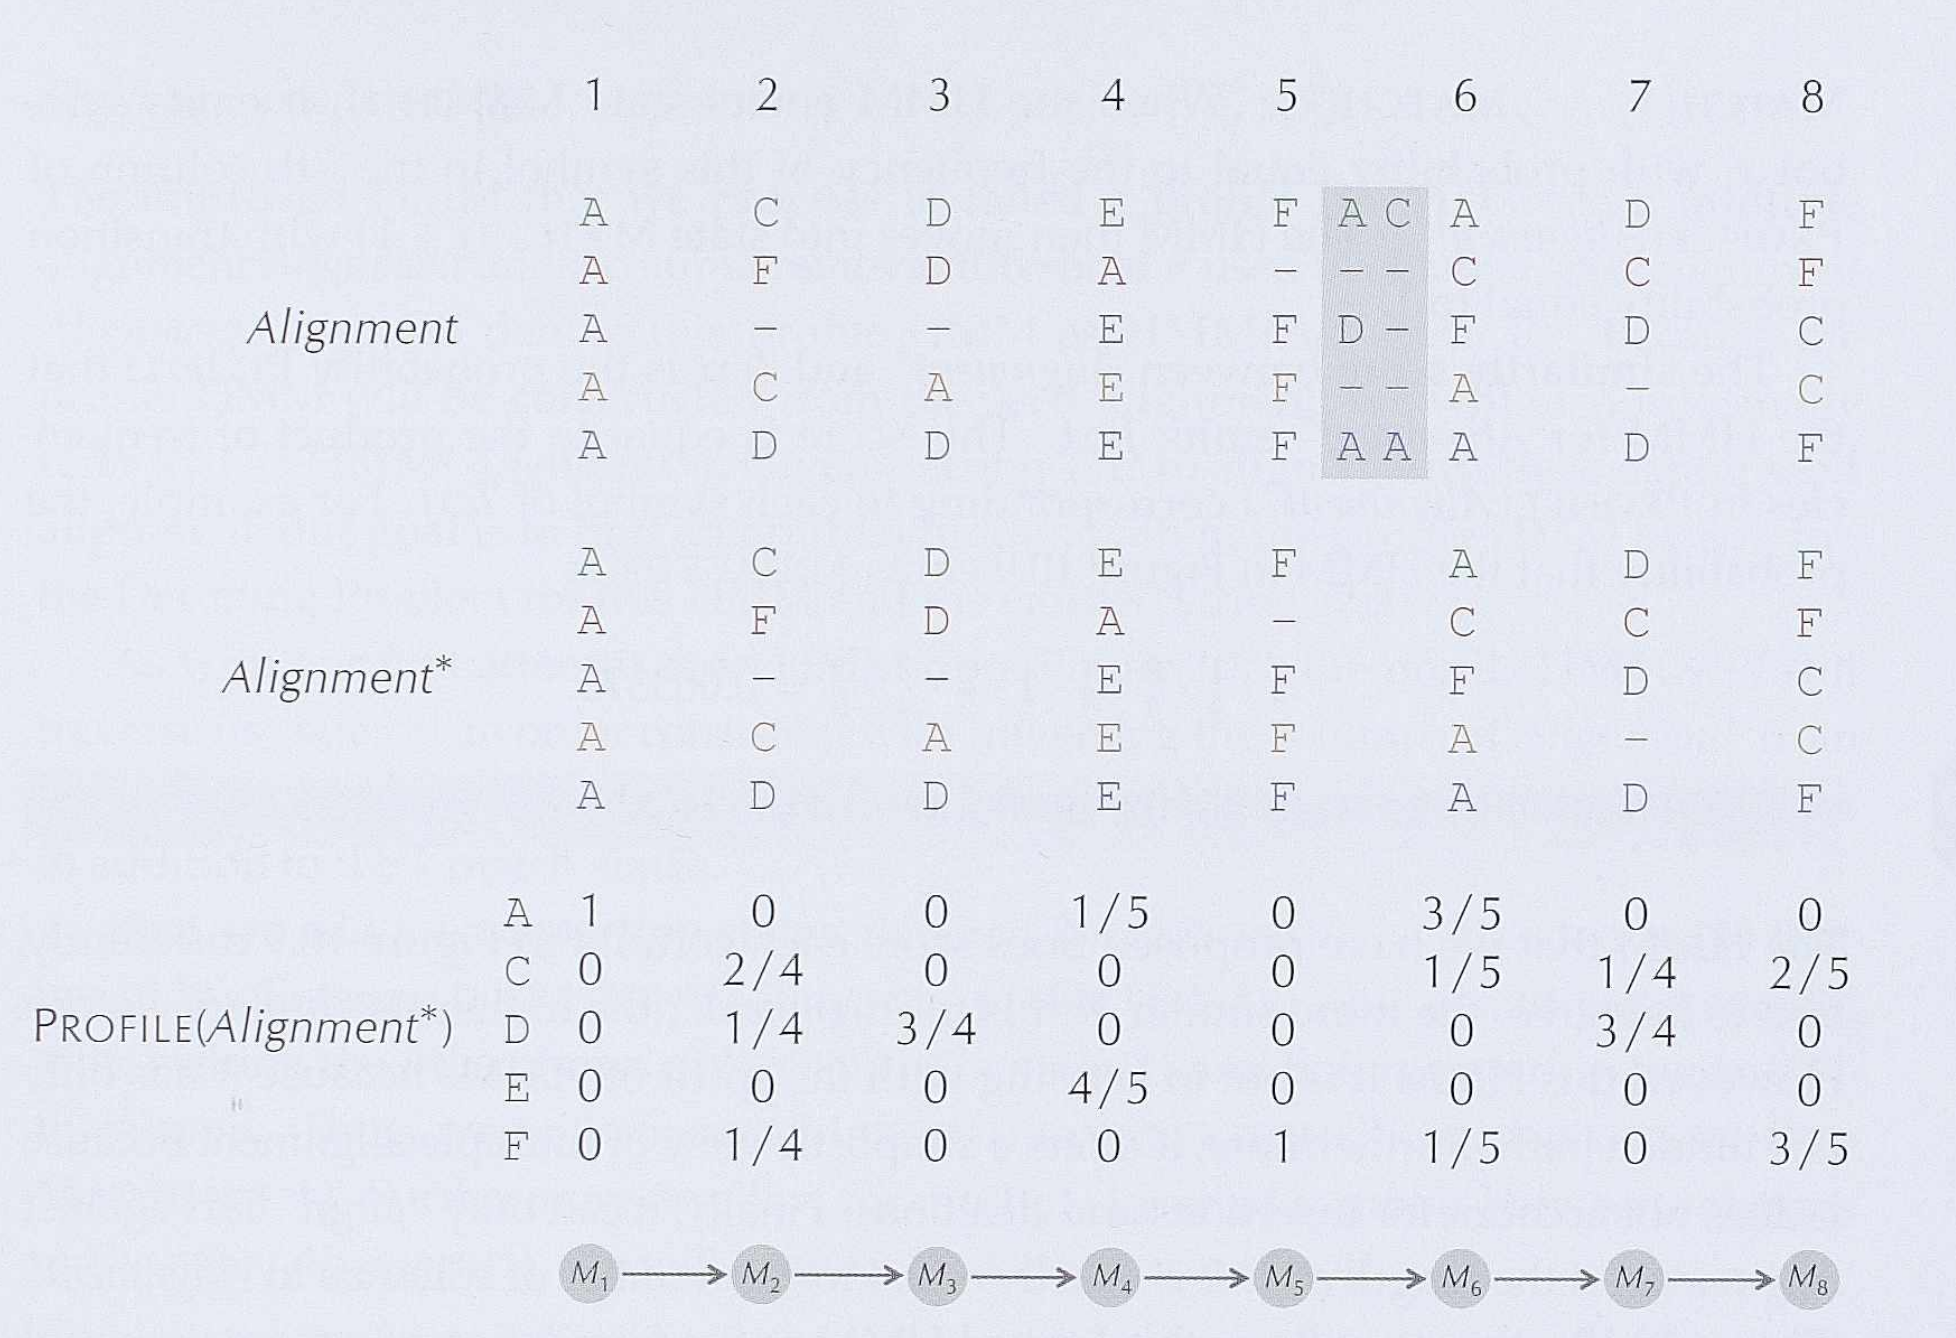
\includegraphics[width=0.8\textwidth]{poglavlja/10/slike/slika1.png}
\caption{5x10 višestruko poravnanje (prvi deo). Uklanjamo kolone ukoliko broj praznina ``-`` prelazi $\theta$. 5x8 semeno poravnanje (drugi deo). Izbacili smo kolone. Profilna matrica semenog poravnanje (treći deo) i jednostavni HMM dijagram koji modelira gornji PROFIL. Semeni algoritam je dobijen od originalnog poravnanja ignorisanjem kolona (osenčenih sivom bojom). U ovom slučaju ignorišemo kolone čiji je deo praznih ``-`` simbola veći ii jednak pragu $\theta$ = 0.35. Kako bismo jasnije prikazali vezu između poravnanja i semenog poravnanja, razdvojili smo prvih 5 kolona u semenom poravnanju od poslednje 3 kolone i numerisali te kolone iznad originalnog poravnanja. Stanja pogotka MATCH(i) su skraćena kao $M_i$. HMM ima samo jednu moguću putanju; u svom početnom stanju MATCH(1), verovatnoća prelaska iz stanja MATCH(i) do stanja MATCH(i+1) je jednaka 1 za svako i svi drugi prelasci su zabranjeni. Emisione verovatnoće su jednake frekvencijama u profilu, npr. emisione verovatnoće za $M_2$ su 0 za A, 2/4 za C, 1/4 za D, 0 za E i 1/4 za F.}
\label{slika: 1}
\end{figure}

da HMM emituje \textit{Text}. Ako je HMM dobro dizajniran, onda što je slicčiji \textit{Text} nizu u \textit{Alignement*}, to će verovatnije biti emitovan od strane HMM-a.

Prvo ćemo konstruisati jednostavan HMM koji tretira kolone \textit{Alignement*-a} kao \textit{k} sekvencijalno povezanih stanja koja ćemo nazvati \textbf{stanja pogotka} (slika \ref{slika: 1} četvrti deo), označeni MATCH(1),...,MATCH(k). Kada HMM uđe u stanje MATCH(i), tada emituje simbol $x_i$ sa verovatnoćom jednakom frekvenciji ovog simbola u i-toj koloni PROFIL(\textit{Alignment*}). HMM se onda prebacuje u stanje MATCH(i+1) sa prelaznom verovatnoćom jednakom 1.

\textbf{Slicnost pogotka} između \textit{Alignment*}-a i \textit{Text}-a je verovatnoća Pr(\textit{Text}) da HMM za \textit{Alignment*} emituje \textit{Text}. Ovaj rezultat je jednak proizvodu frekvencija u PROFILE(\textit{Alignment*}) koji odgovaraju svakom simbolu iz \textit{Text}-a. Na primer, verovatnoća da HMM na slici \ref{slika: 1} emituje ADDAFFDF je:
\begin{equation}
    1 \cdot \frac{1}{4} \cdot \frac{3}{4} \cdot \frac{1}{5} \cdot 1 \cdot \frac{1}{5} \cdot \frac{3}{4} \cdot \frac{3}{5} = 0.003375.
\end{equation}

HMM koji smo prikazali rezultuje svaku kolonu na slici \ref{slika: 1} drugačije i do određenog stepena, što je sličniji \textit{Text} \textit{Alignment*}-u, to je veći rezultat sličnosti. Međutim, ovaj HMM ima samo jednu skrivenu putanju, i nudi jednostavan pogled višestrukih poravnanja zato što ne uracunava inserciju i brisanja. Na kraju, \textit{Text} se može ``poravnati`` u odnosu na \textit{Alignment*} ako je dužina \textit{Text}-a tačno jednaka broju kolona u \textit{Alignment*}-u (slika \ref{slika: 2}). Ipak mi ćemo iskoristiti ovaj ograničeni HMM kao temelj za moćnije HMM-ove.

\begin{figure}[H]
\centering
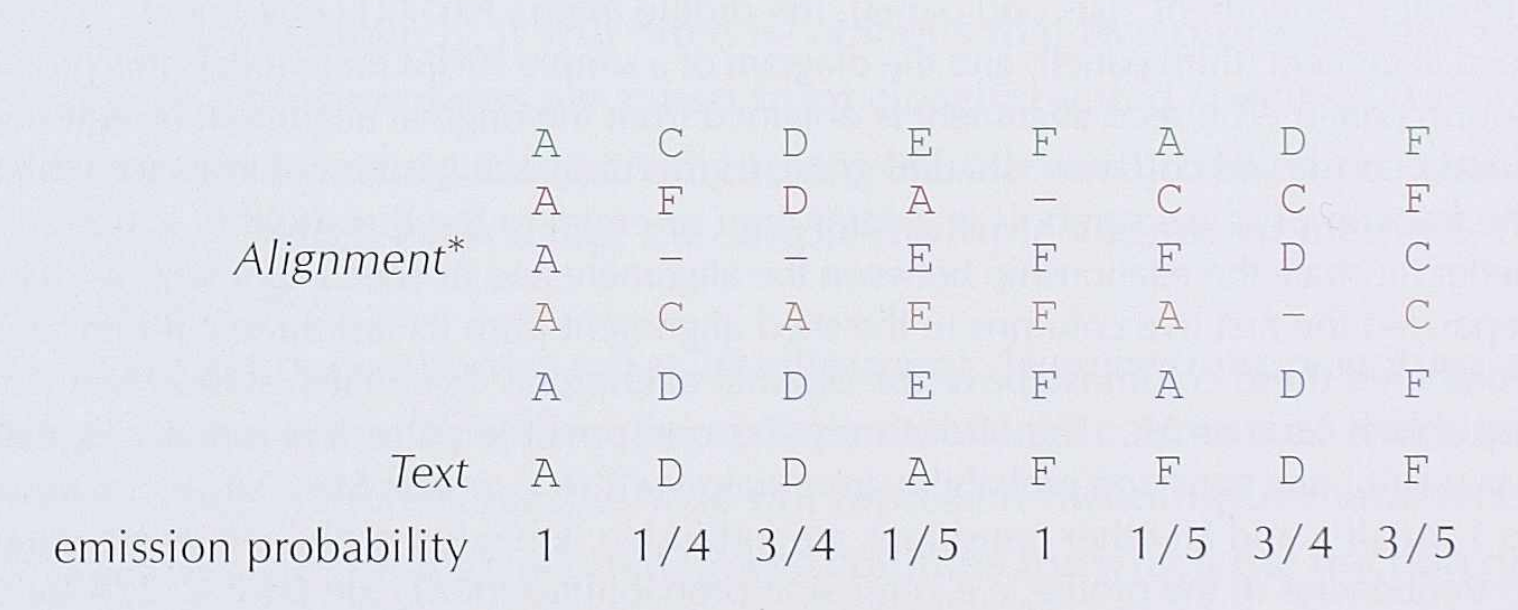
\includegraphics[width=0.8\textwidth]{poglavlja/10/slike/slika2.png}
\caption{Poravnanje Text = ADDAFFDF u odnosu na semeno poravnanje \textit{Alignment*} predstavljeno kao jednostavan HMM na slici \ref{slika: 1}. Ovaj HMM je ograničen zato što nismo u mogućnosti da poravnamo nizove dužine različite od 8. }
\label{slika: 2}
\end{figure}

\subsection{Građenje profilnog HMM-a}

Poboljšani HMM koji cemo predstaviti se zove \textbf{profilni HMM}. Sa datim višestrukim poravnanjem \textit{Alignment} i pragom brisanja kolona $\theta$ koji koristimo da dođemo do \textit{Alignment*}-a, označićemo ovaj profilni HMM kao HMM(\textit{Alignment, $\theta$}). Za dati niz \textit{Text} da se poravna u odnosu na postojeće semeno poravnanje, naš cilj je da pronađemo optimalni skriveni put u profilnom HMM-u tako što ćemo rešiti Problem Dekodiranja za ovaj HMM i emitovani niz \textit{Text}.

Prvo dodajemo $ k+1 $ \textbf{insercionih stanja}, označenih kao INSERTION(0),...,INSERTION($ k $) (slika \ref{slika: 3}). Ulaženje u INSERTION($ i $) dopušta profilnom HMM-u da emituje dodatni simbol nakon posećivanja $ i $-te kolone PROFILE(\textit{Alignment*})-a i pre ulaženja u $ (i+1) $-tu kolonu. Povezujemo MATCH($ i $) sa INSERTION($ i $) i INSERTION($ i $) sa MATCH($ i+1 $). Kako bismo dopustili višestruke insertovane simbole između kolona PROFILE(\textit{Alignment*})-a, povezaćemo INSERTION($ i $) samu sa sobom.

\begin{figure}[H]
\centering
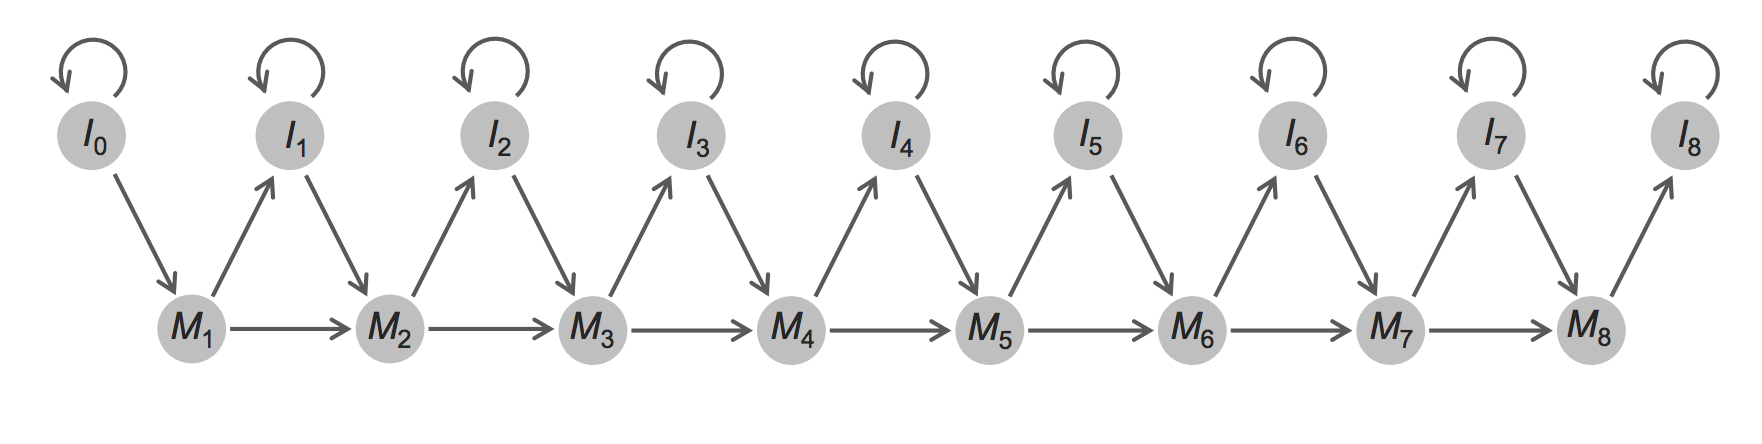
\includegraphics[width=0.8\textwidth]{poglavlja/10/slike/slika3.png}
\caption{HMM dijagram za semeno poravnanje sa slike \ref{slika: 1} sa pogotcima i insercionim stanjima, skraćeni kao M i I, redom. Stanja $I_0$ i $I_8$ modeluju insercije simbola koje se dešavaju pre početka i kraja \textit{Alignment*}-a, redom.}
\label{slika: 3}
\end{figure}

\textbf{Pitanje}: Da li možemo da iskoristimo HMM na slici \ref{slika: 3} da poravnamo niz \textit{Text} dužine manje od 8?

Nakon modelovanja insercija novih simbola u PROFILE(\textit{Alignment*}), treba da modelujemo i ``delecije`` koja omogućavaju profilnom HMM-u da preskoči kolone PROFILE(\textit{Alignment*})-a. Jedan način modeliranja ovih delecija je da dodamo ivice koje povezuju svako stanje u profilnom HMM-u sa svakim stanjem desno od njega (slika \ref{slika: 4}).

\begin{figure}[H]
\centering
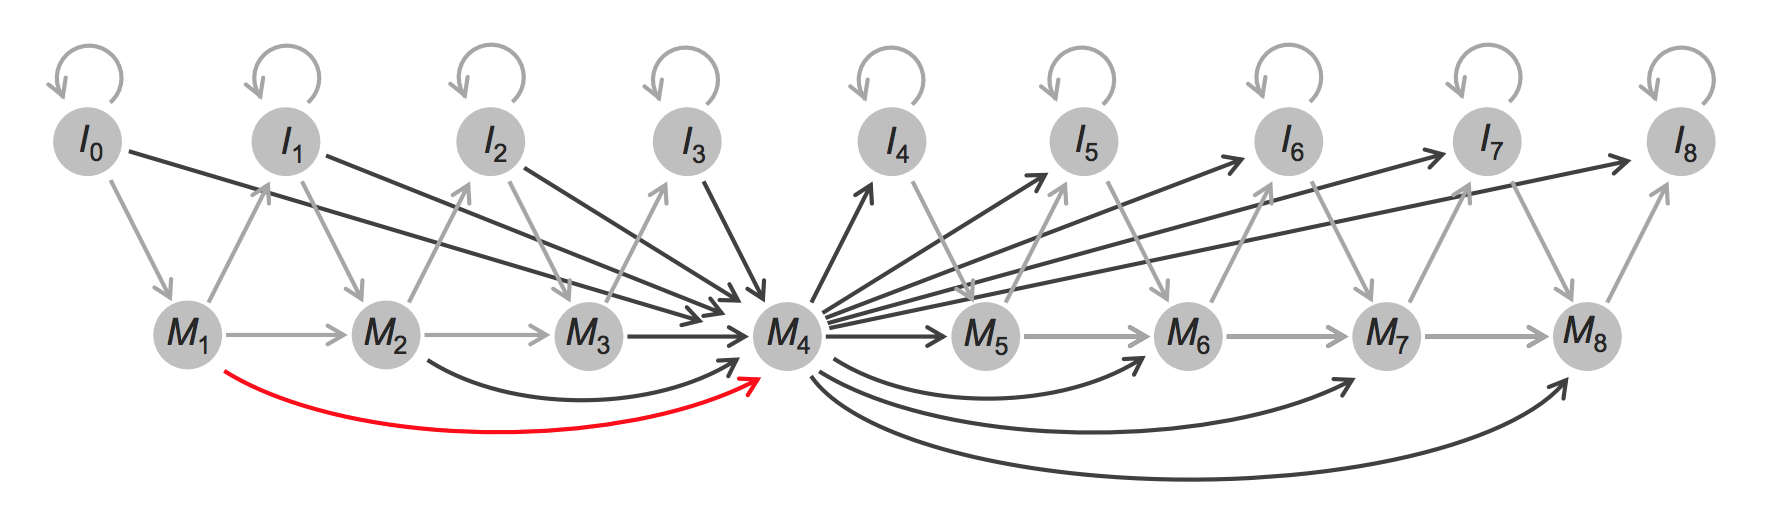
\includegraphics[width=0.8\textwidth]{poglavlja/10/slike/slika4.png}
\caption{Dodavanjem ivica koje povezuju svako stanje u profilnom HMM-u sa slike \ref{slika: 3} sa svakim stanjem desno od njega, možemo preskočiti kolone \textit{Alignment}-a kada poredimo \textit{Text} u odnosu na ovo poravnanje. Gornji HMM dijagram označava da sve ivice vode u i iz MATCH(4).}
\label{slika: 4}
\end{figure}

\begin{figure}[H]
\centering
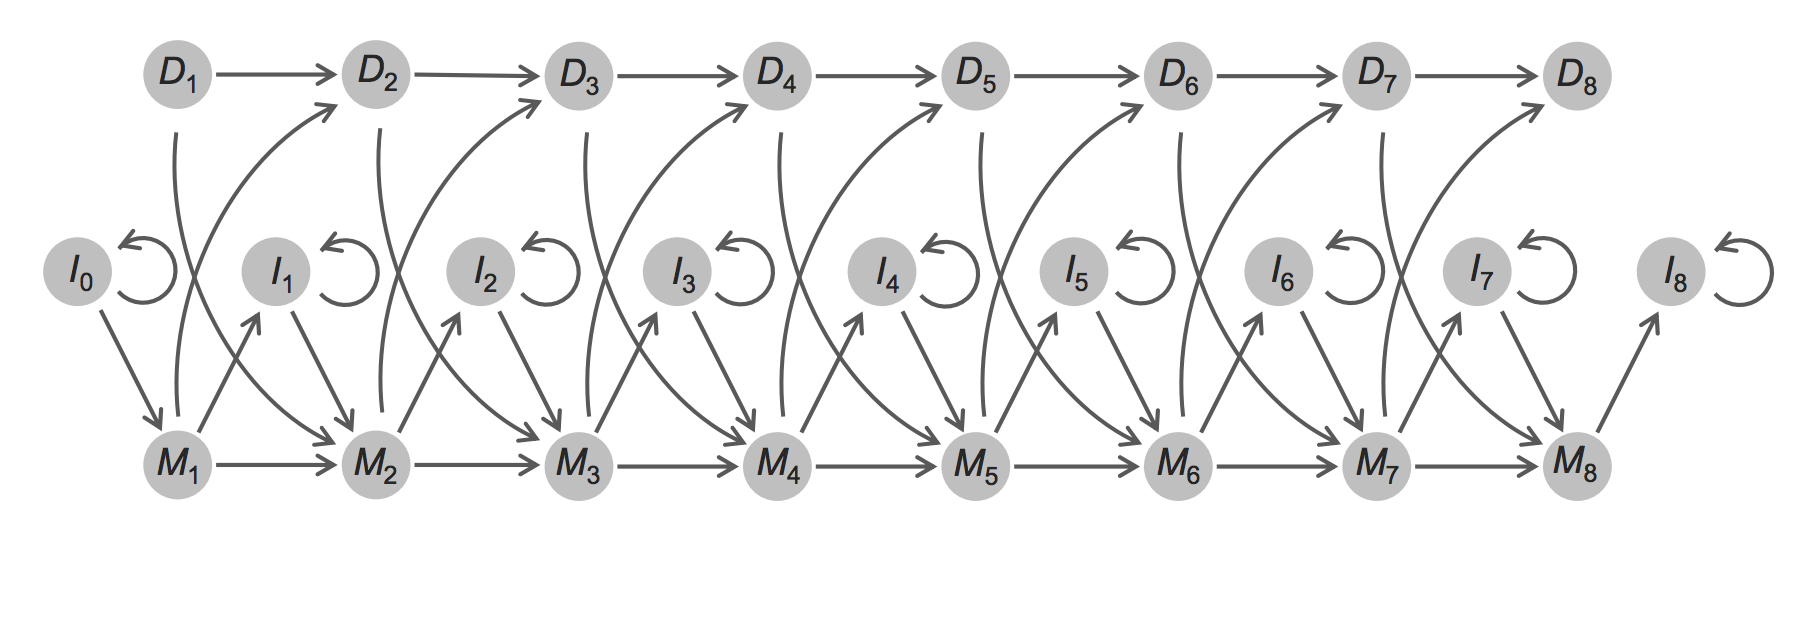
\includegraphics[width=0.8\textwidth]{poglavlja/10/slike/slika5.png}
\caption{Dodavanje stanja deleciji (skraceno kao $D_i$) profilnom HMM dijagramu.}
\label{slika: 5}
\end{figure}

\begin{figure}[H]
\centering
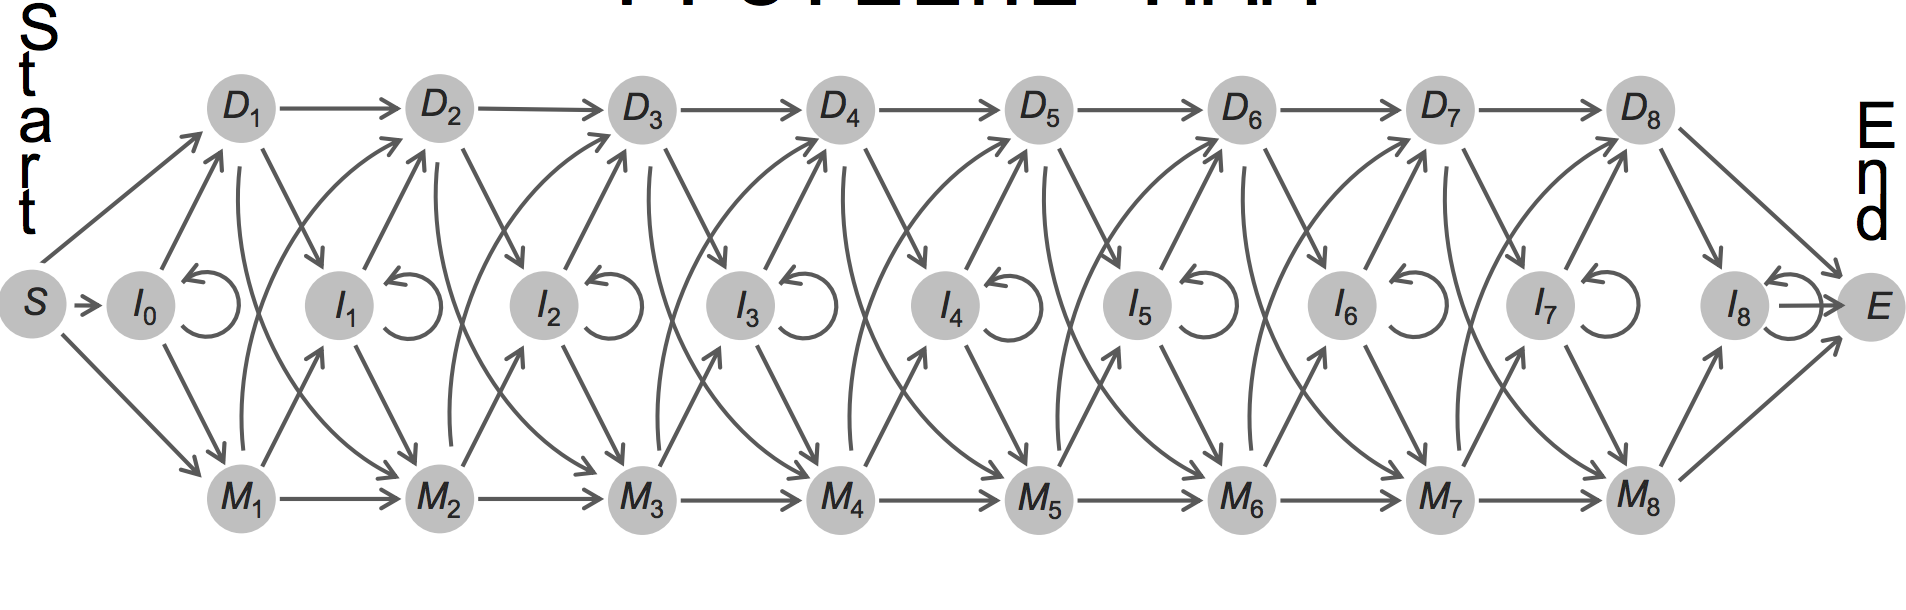
\includegraphics[width=0.8\textwidth]{poglavlja/10/slike/slika6.png}
\caption{Dodavanje prelaza od insercionih stanja do delecionih stanja i obrnuto upotpunjava profilni HMM dijagram za profilnu matricu na slici \ref{slika: 1}. Početno i završno stanje su označeno kao S i E, redom.}
\label{slika: 6}
\end{figure}

\begin{problem}[Problem profilnog HMM-a ]
	Konstruisati profilni HMM na osnovu višestrukog poravnanja.\\
	Ulaz: Višestruko poravnanje \textit{Alignment} i parametar $\theta$
(maksimalni udeo insercija po koloni). \\
	Izlaz: Emisiona i tranziciona matrica profilnog HMM HMM(\textit{Alignment,$\theta$}). 
\end{problem}

\begin{figure}[H]
\centering
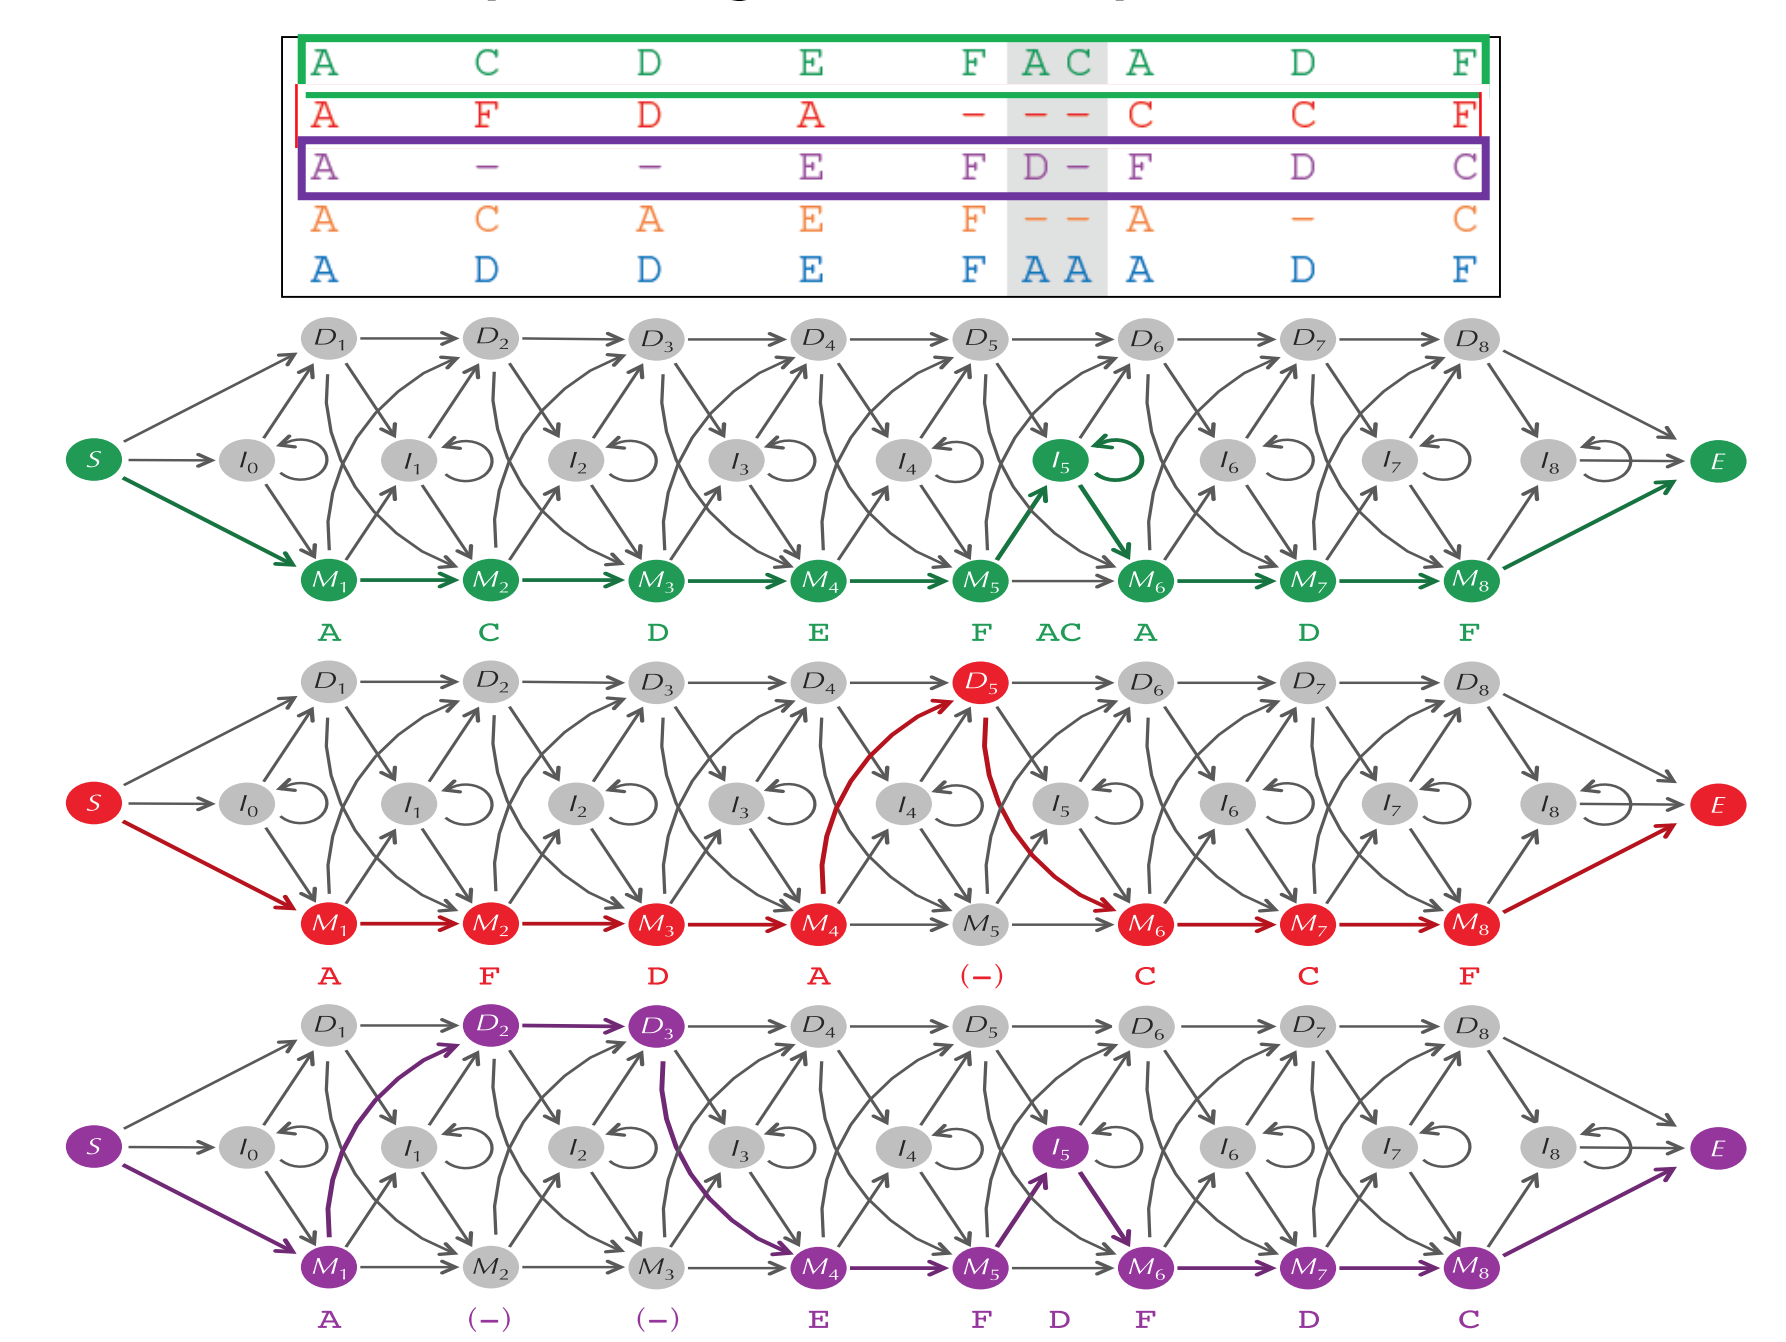
\includegraphics[width=0.8\textwidth]{poglavlja/10/slike/slika7.png}
\caption{Tri putanje kroz profilni HMM koje odgovaraju trima redovima i poravnanju na slici \ref{slika: 1}. Prazni simboli ``-`` ispod HMM dijagrama koji odgovaraju delecionim stanjima su prikazani u zagradama da naznače da se ne emituju od strane HMM-a}
\label{slika: 7}
\end{figure}

\begin{figure}[H]
\centering
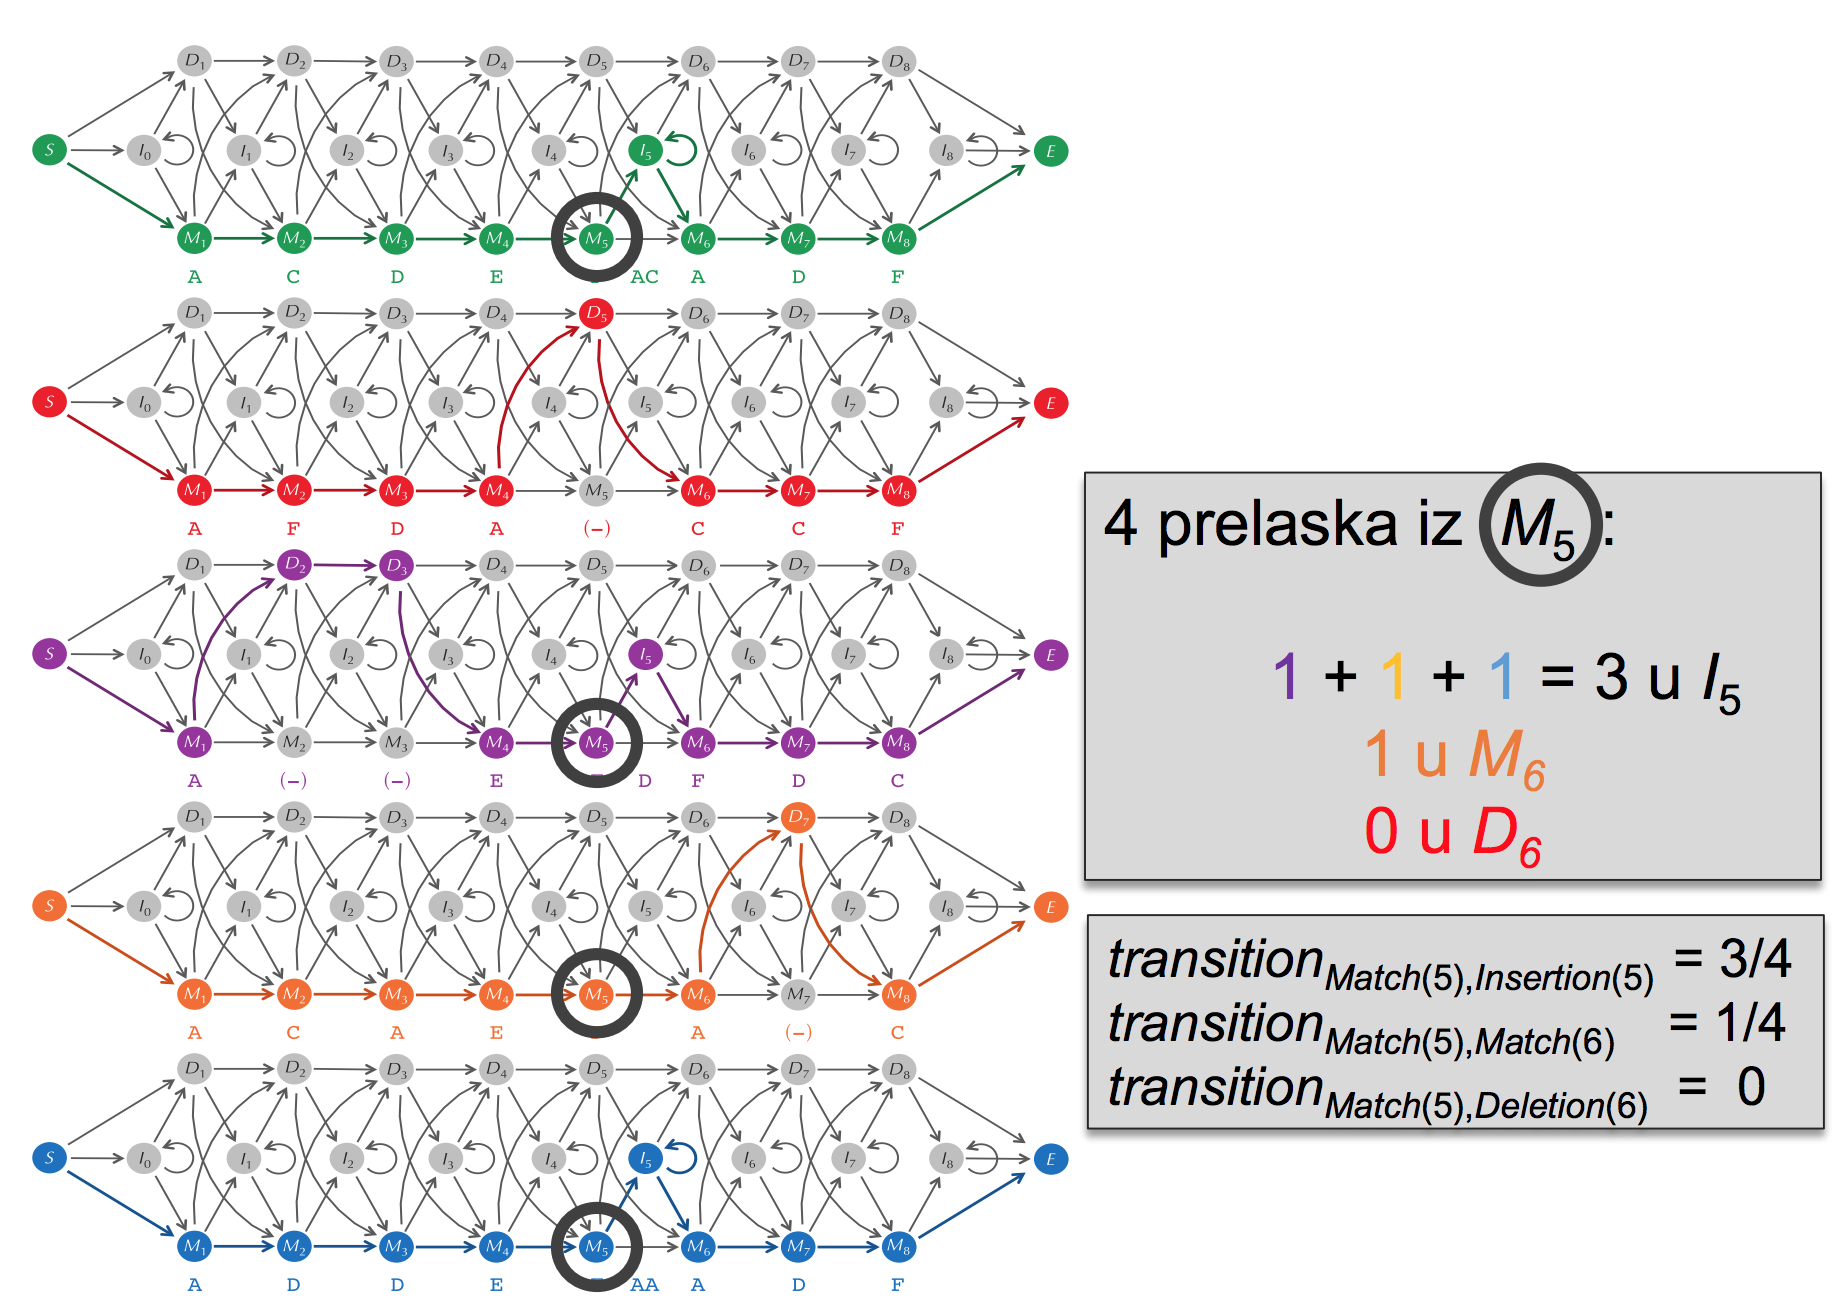
\includegraphics[width=0.8\textwidth]{poglavlja/10/slike/slika8.png}
\caption{Verovatnoće prelaska u profilnom HMM}
\label{slika: 8}
\end{figure}

\begin{figure}[H]
\centering
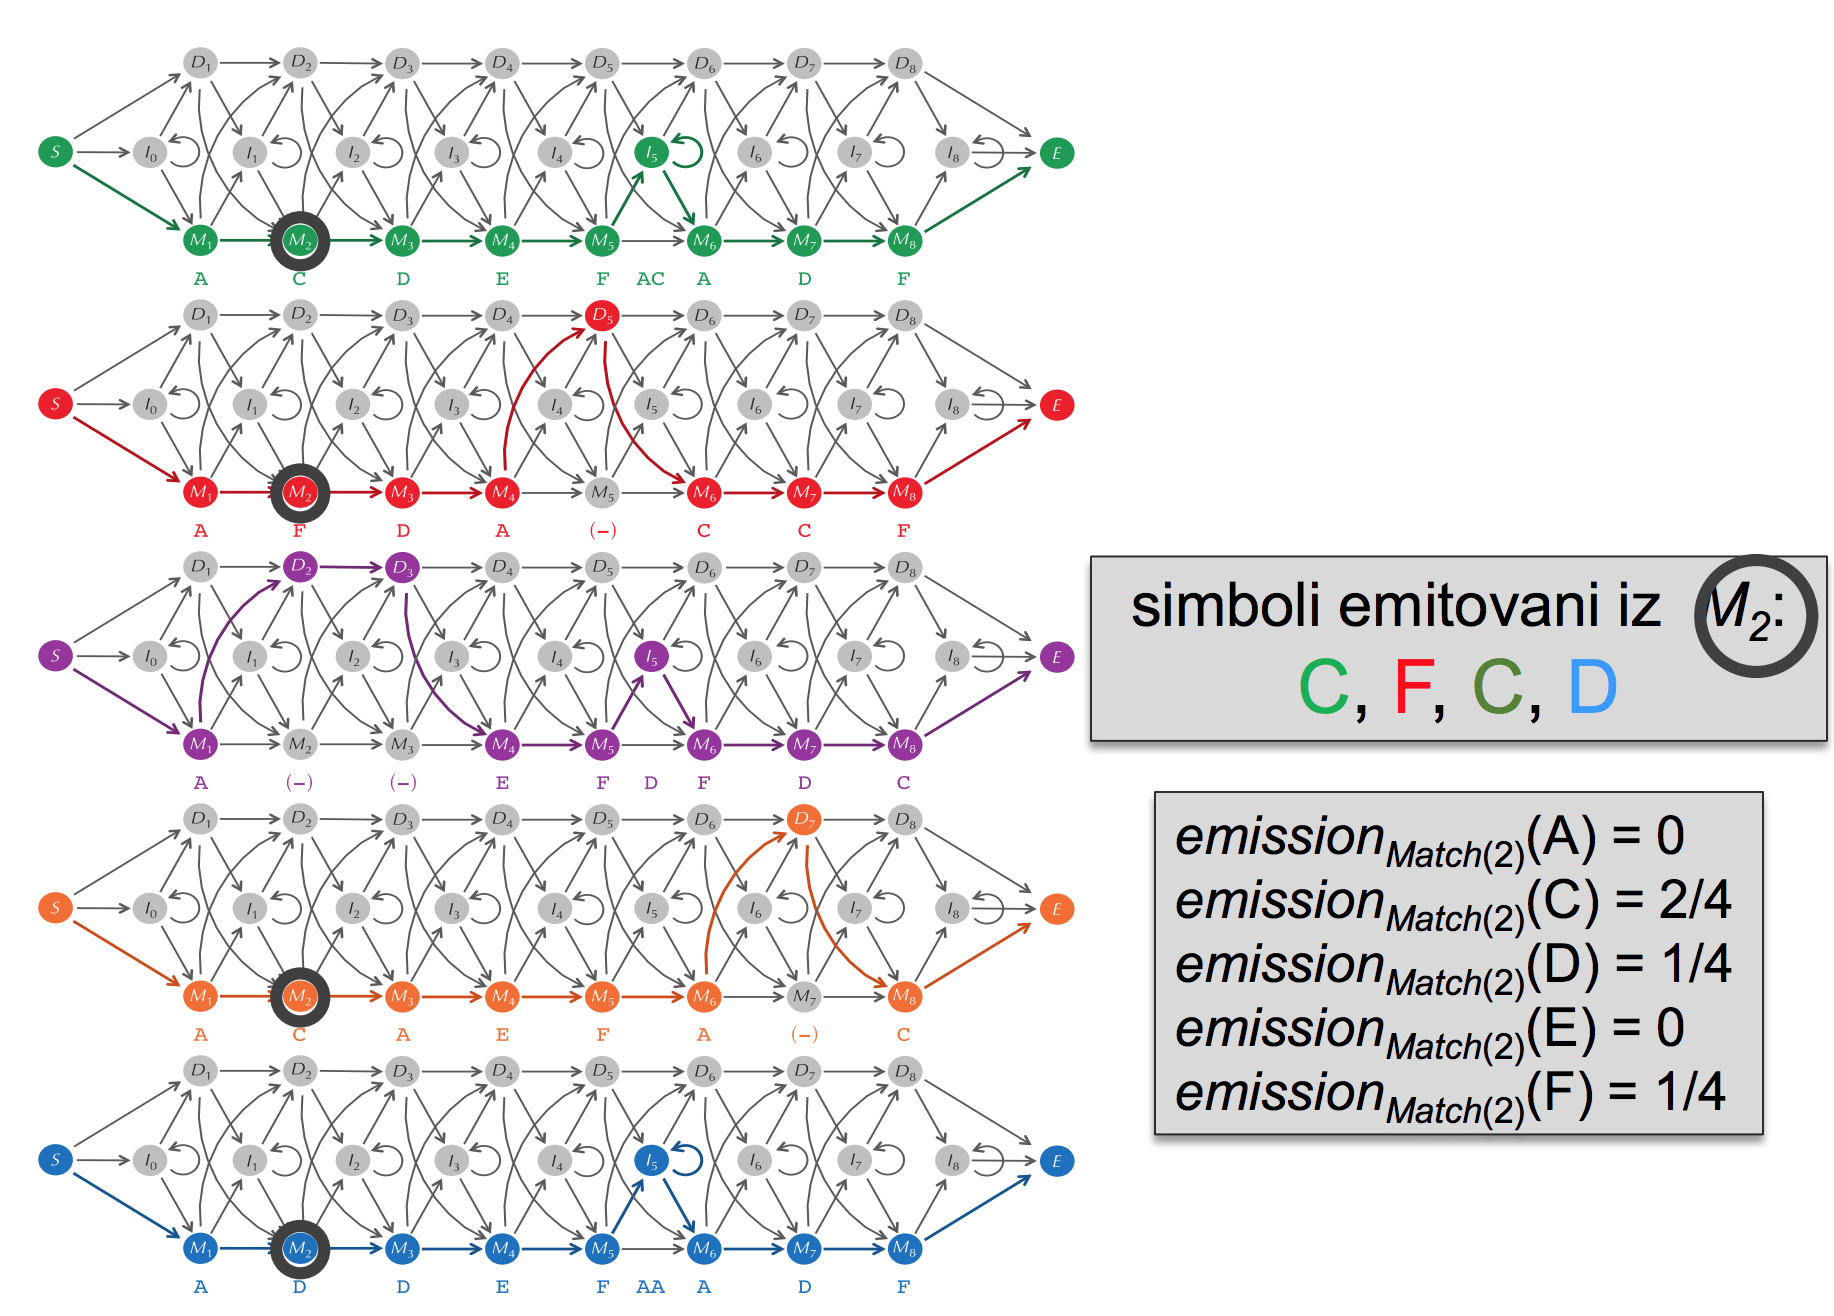
\includegraphics[width=0.8\textwidth]{poglavlja/10/slike/slika9.png}
\caption{Emisione verovatnoće u profilnom HMM}
\label{slika: 9}
\end{figure}

\begin{figure}[H]
\centering
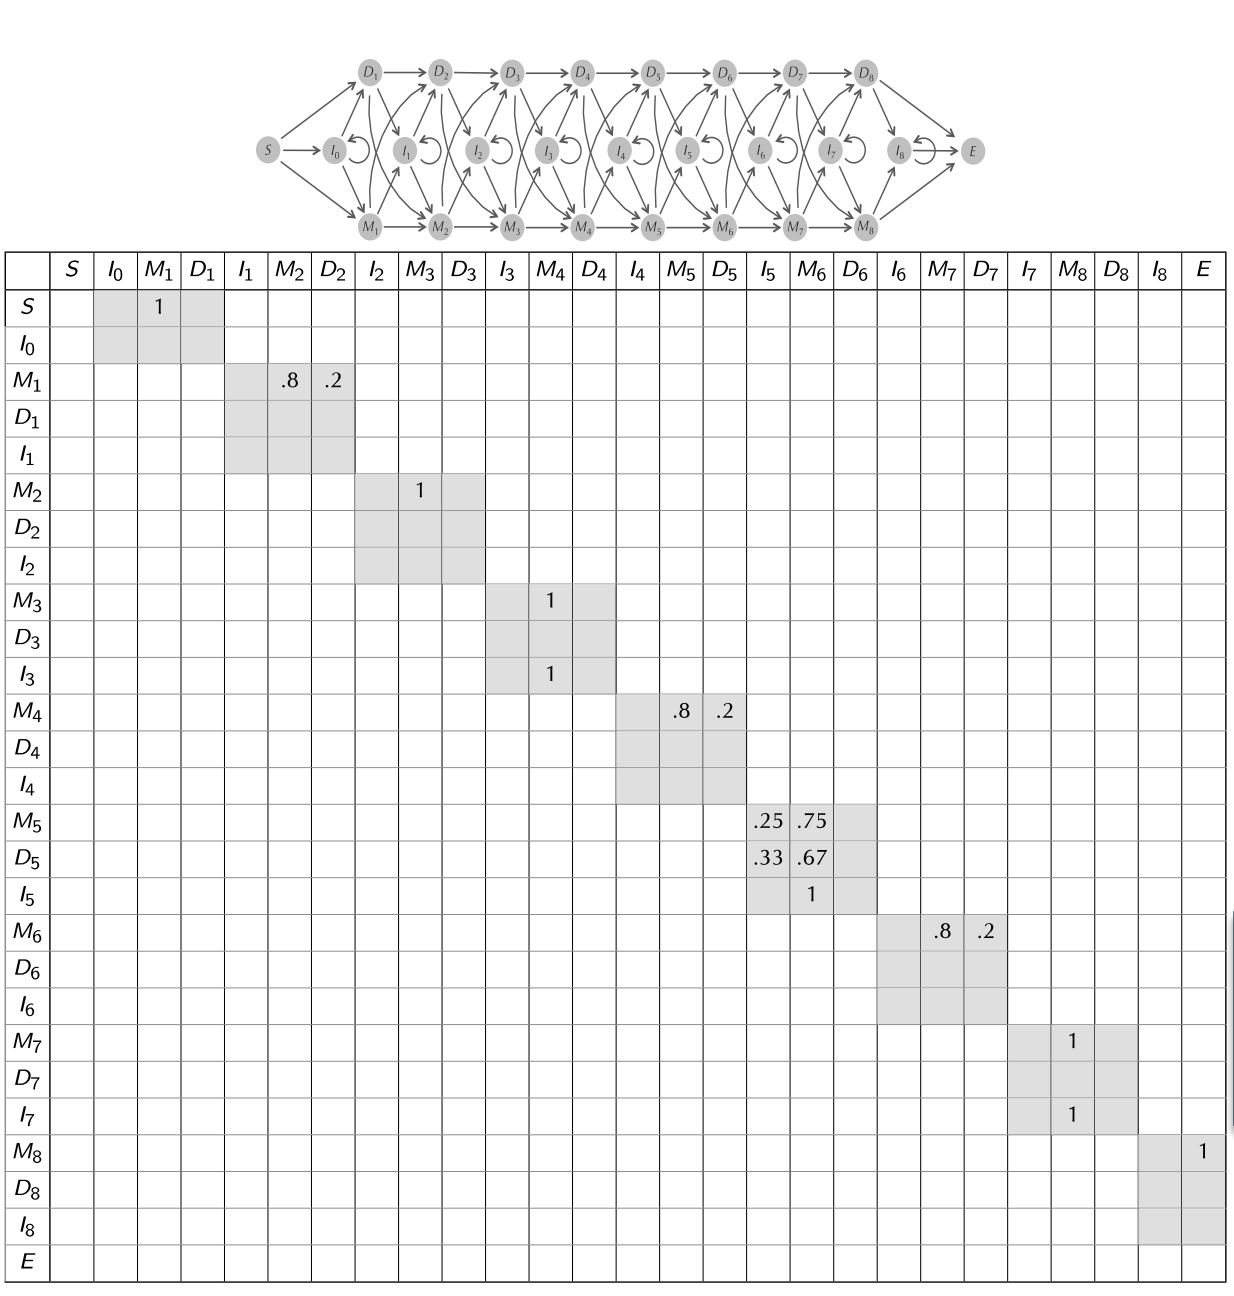
\includegraphics[width=0.8\textwidth]{poglavlja/10/slike/slika10.png}
\caption{Zabranjeni prelasci. \textbf{Sive ćelije}: grane u HMM dijagramu. \textbf{Prazne ćelije}: zabranjeni prelasci.}
\label{slika: 10}
\end{figure}

\section{Zadaci sa vežbi}

U nastavku će biti predstavljeni zadaci sa vežbi na kursu rađeni u programskom jeziku Python.

\subsection{HMM}

\lstinputlisting[language=Python]{poglavlja/10/kodovi/1.py}
